% Options for packages loaded elsewhere
\PassOptionsToPackage{unicode}{hyperref}
\PassOptionsToPackage{hyphens}{url}
%
\documentclass[
  12pt,
]{article}
\usepackage{amsmath,amssymb}
\usepackage{lmodern}
\usepackage{iftex}
\ifPDFTeX
  \usepackage[T1]{fontenc}
  \usepackage[utf8]{inputenc}
  \usepackage{textcomp} % provide euro and other symbols
\else % if luatex or xetex
  \usepackage{unicode-math}
  \defaultfontfeatures{Scale=MatchLowercase}
  \defaultfontfeatures[\rmfamily]{Ligatures=TeX,Scale=1}
\fi
% Use upquote if available, for straight quotes in verbatim environments
\IfFileExists{upquote.sty}{\usepackage{upquote}}{}
\IfFileExists{microtype.sty}{% use microtype if available
  \usepackage[]{microtype}
  \UseMicrotypeSet[protrusion]{basicmath} % disable protrusion for tt fonts
}{}
\makeatletter
\@ifundefined{KOMAClassName}{% if non-KOMA class
  \IfFileExists{parskip.sty}{%
    \usepackage{parskip}
  }{% else
    \setlength{\parindent}{0pt}
    \setlength{\parskip}{6pt plus 2pt minus 1pt}}
}{% if KOMA class
  \KOMAoptions{parskip=half}}
\makeatother
\usepackage{xcolor}
\IfFileExists{xurl.sty}{\usepackage{xurl}}{} % add URL line breaks if available
\IfFileExists{bookmark.sty}{\usepackage{bookmark}}{\usepackage{hyperref}}
\hypersetup{
  pdftitle={Voxel-wise Intermodal Coupling Analysis of Two or More Modalities using Local Covariance Decomposition},
  hidelinks,
  pdfcreator={LaTeX via pandoc}}
\urlstyle{same} % disable monospaced font for URLs
\usepackage[margin=1in]{geometry}
\usepackage{longtable,booktabs,array}
\usepackage{calc} % for calculating minipage widths
% Correct order of tables after \paragraph or \subparagraph
\usepackage{etoolbox}
\makeatletter
\patchcmd\longtable{\par}{\if@noskipsec\mbox{}\fi\par}{}{}
\makeatother
% Allow footnotes in longtable head/foot
\IfFileExists{footnotehyper.sty}{\usepackage{footnotehyper}}{\usepackage{footnote}}
\makesavenoteenv{longtable}
\usepackage{graphicx}
\makeatletter
\def\maxwidth{\ifdim\Gin@nat@width>\linewidth\linewidth\else\Gin@nat@width\fi}
\def\maxheight{\ifdim\Gin@nat@height>\textheight\textheight\else\Gin@nat@height\fi}
\makeatother
% Scale images if necessary, so that they will not overflow the page
% margins by default, and it is still possible to overwrite the defaults
% using explicit options in \includegraphics[width, height, ...]{}
\setkeys{Gin}{width=\maxwidth,height=\maxheight,keepaspectratio}
% Set default figure placement to htbp
\makeatletter
\def\fps@figure{htbp}
\makeatother
\setlength{\emergencystretch}{3em} % prevent overfull lines
\providecommand{\tightlist}{%
  \setlength{\itemsep}{0pt}\setlength{\parskip}{0pt}}
\setcounter{secnumdepth}{5}
\newlength{\cslhangindent}
\setlength{\cslhangindent}{1.5em}
\newlength{\csllabelwidth}
\setlength{\csllabelwidth}{3em}
\newlength{\cslentryspacingunit} % times entry-spacing
\setlength{\cslentryspacingunit}{\parskip}
\newenvironment{CSLReferences}[2] % #1 hanging-ident, #2 entry spacing
 {% don't indent paragraphs
  \setlength{\parindent}{0pt}
  % turn on hanging indent if param 1 is 1
  \ifodd #1
  \let\oldpar\par
  \def\par{\hangindent=\cslhangindent\oldpar}
  \fi
  % set entry spacing
  \setlength{\parskip}{#2\cslentryspacingunit}
 }%
 {}
\usepackage{calc}
\newcommand{\CSLBlock}[1]{#1\hfill\break}
\newcommand{\CSLLeftMargin}[1]{\parbox[t]{\csllabelwidth}{#1}}
\newcommand{\CSLRightInline}[1]{\parbox[t]{\linewidth - \csllabelwidth}{#1}\break}
\newcommand{\CSLIndent}[1]{\hspace{\cslhangindent}#1}
\usepackage{booktabs}
\ifLuaTeX
  \usepackage{selnolig}  % disable illegal ligatures
\fi
\usepackage[]{natbib}
\bibliographystyle{plainnat}

\title{Voxel-wise Intermodal Coupling Analysis of Two or More Modalities using Local Covariance Decomposition}
\author{true \and true \and true \and true \and true \and true \and true \and true \and true \and true \and true \and true \and true \and true \and true \and true \and true}
\date{02 January, 2022}

\begin{document}
\maketitle

{
\setcounter{tocdepth}{2}
\tableofcontents
}
\hypertarget{credit-author-statement}{%
\section{CRediT author statement}\label{credit-author-statement}}

Fengling Hu: Conceptualization, Methodology, Software, Validation, Formal analysis, Investigation, Writing - Original Draft, Writing - Review \& Editing, Visualization

TODO

\url{https://www.elsevier.com/authors/policies-and-guidelines/credit-author-statement}

\hypertarget{abstract}{%
\section{Abstract}\label{abstract}}

When individual subjects undergo imaging with multiple modalities, biological information is present not only within each modality, but also between modalities - that is, in how modalities covary at the voxel level. Previous studies have shown that the covariance structures between modalities, or intermodal coupling (IMCo), can be estimated between two modalities, and that two-modality IMCo reveals otherwise undiscovered patterns in neurodevelopment as well as other processes. However, previous IMCo methods are based on the slopes of local weighted linear regression lines, which are inherently asymmetric and limited to the two-modality setting. Here, we present a PCA-based generalization of IMCo regression which uses local covariance decompositions to define a symmetric, voxel-wise coupling coefficient valid for two or more modalities. We then use this method to study coupling between cerebral blood flow, resting state activations, and functional connectivity in 803 subjects between ages 8 and 23. We demonstrate that coupling is spatially heterogeneous and varies with respect to age and sex over the course of neurodevelopment. As availability of multi-modal data increases, PCA-based IMCo offers a natural approach for summarizing relationships between multiple aspects of brain structure and function. An R package is provided.

\hypertarget{introduction}{%
\section{Introduction}\label{introduction}}

There is increased availability of multi-modality neuroimaging data on individual subjects, where each modality contains unique information about brain structure or function {[}TOCITE{]}. Such data allow us to explore patternss in individual modalities and how patterns in individual modalities relate to each other. In addition to these comparisons, multi-modal data allows us to observe the local covariance structure, or intermodal coupling (IMCo), between modalities \citep{ballerDevelopmentalCouplingCerebral2021, valcarcelMIMoSAAutomatedMethod2018, vandekarSubjectlevelMeasurementLocal2016}. This local covariance structure can be interpreted as how modalities relate with respect to one another at the voxel level in individual subjects.

Previous studies have shown IMCo analysis is complementary to single-modality analysis and unveils otherwise undetectable findings {[}TOCITE{]}. For example, in neurodevelopment, IMCo between cortical thickness and sulcal depth has suggested the cortical sheet is generally thinner in sulcal locations when compared to gyral locations, though this relationship was more spatially heterogeneous than previously described \citep{vandekarSubjectlevelMeasurementLocal2016}. Additionally, this study showed the strength of coupling was lower in males compared to females and decreased with age. A separate study exploring IMCo between cerebral blood flow and amplitude of low frequency fluctuations (ALFF) showed that age-related declines in neurovascular coupling occurred most drastically during mid-adolescence and were enriched in the dorsal attention network \citep{ballerDevelopmentalCouplingCerebral2021}. There were also differences in CBF-ALFF coupling between males and females; these differences were enriched in the frontoparietal network. In multiple sclerosis, IMCo has also shown use as a data augmentation tool to improve predictive accuracy of an automated lesion detection model over models using individual modality data alone \citep{valcarcelDualModelingApproach2018, valcarcelMIMoSAAutomatedMethod2018}.

In these prior studies, each voxel-wise coupling value was defined as the slope of the weighted regression lines fit within a local neighborhood between two modalities. However, since this method of calculating IMCo is based on regression slopes, it does not take into account voxel-level correlation and also suffers from inherent asymmetry, where coupling values depend on the order in which modalities are listed. For example, depending on which modality is the reference modality, a coupling value, \(m\), will change to its inverse, \(1 / m\); this issue is especially problematic for coupling values with very small or very large magnitudes. Thus, this asymmetry necessitates arbitrary, yet influential, decision-making when it comes to analysis and inhibits straight-forward interpretation. Such a measure for IMCo is also limited to only two modalities, so the study of coupling between more than two modalities would require analysis of all pairwise coupling maps. As the number of total modalities increase, this can quickly become overwhelming to interpret.

We propose a novel, principal component analysis (PCA) based method for estimating IMCo that uses local covariance decomposition to define symmetric voxel-wise coupling values valid for two or more modalities that reduce the complex local covariance structures into a single value. Thus, our approach provides a more natural and interpretable way of describing coupling in settings with two modalities and allows for simplified study of overall local covariance structure in settings with more than two modalities. To demonstrate its sensitivity to biologically relevant patterns, we show PCA-based IMCo uncovers differences in three-modality coupling with respect to age and sex throughout neurodevelopment.

\hypertarget{methods}{%
\section{Methods}\label{methods}}

\hypertarget{subjects}{%
\subsection{Subjects}\label{subjects}}

We included 803 subjects (340 males) from ages 8-23 (mean = 15.6; sd = 3.3) from the Philadelphia Neurodevelopmental Cohort (PNC) \citep{satterthwaite_neuroimaging_2014}. Of the 1445 PNC subjects who underwent neuroimaging, we initially excluded those meeting any of the following criteria: history of psychoactive medication (n = 165), history of inpatient psychiatric hospitalization (n = 51), or history of medical disorders that could impact brain function (n = 166). From the remaining 1113 subjects, we included those who underwent the combination of T1-weighted MRI, arterial spin labeling MRI (ASL), and resting state fMRI (rfMRI) scanning, each of acceptable image quality as determined based on automated and manual screening. This resulted in the final set of 803 subjects used for this study.

The Institutional Review Boards of the University of Pennsylvania and the Children's Hospital of Pennsylvania approved all study procedures. All study subjects gave informed consent; for subjects under the age of 18, parents or guardians provided consent and subjects provided assent. Additional details of the PNC study have been previously described \citep{satterthwaite_neuroimaging_2014}.

\hypertarget{image-acquisition}{%
\subsection{Image acquisition}\label{image-acquisition}}

All PNC imaging was acquired using a single 3T Siemens Tim Trio scanner with a 32-channel head coil. To minimize motion, subject heads stabilized using one foam pad over each ear and one over the top of the head. Image acquisition procedures have been previously described \citep{satterthwaite_neuroimaging_2014}.

T1 structural images were used for alignment of all scans into common space. T1 images by 3D-encoded magnetization-prepared, rapid acquisition gradient echo (MPRAGE) T1-weighted sequence with the following settings: \(T_R\) = 1810 ms; \(T_E\) = 3.51 ms; FoV = 180 × 240 mm; matrix size = 192 x 256; number of slices = 160; slice thickness = 1 mm; inter-slice gap = 0 mm; resolution = 0.9375 × 0.9375 × 1 mm. Cerebral blood flow (CBF) was estimated from a 3D-encoded spin-echo pseudo-continuous arterial spin labeling (pCASL) sequence with the following settings: \(T_R\) = 4000 ms; \(T_E\) = 15 ms; FoV = 220 × 220 mm; matrix size = 96 x 96; number of slices = 20; slice thickness = 5 mm; inter-slice gap = 1 mm; resolution = 2.3 x 2.3 x 6 mm; 80 volumes. Maps of amplitude of low frequency fluctuations (ALFF) and regional homogeneity (ReHo) were estimated from six minutes of task-free functional data from a blood oxygen level-dependent (BOLD-weighted) 2D EPI sequence with the following settings: \(T_R\) = 3000 ms; \(T_E\) = 32 ms; FoV = 192 × 192 mm; matrix size = 64 x 64; number of slices = 46; slice thickness = 3 mm; inter-slice gap = 0 mm; resolution = 3 mm isotropic; 124 volumes. Subjects were instructed to stay awake, keep their eyes open and fixated on a displayed fixation cross, and remain still.

\hypertarget{image-processing}{%
\subsection{Image processing}\label{image-processing}}

TODO

\hypertarget{estimation-of-intermodal-coupling}{%
\subsection{Estimation of intermodal coupling}\label{estimation-of-intermodal-coupling}}

For each subject, we calculated voxel-wise IMCo between CBF, ALFF, and ReHo modalities. Even though ALFF and ReHo are technically calculated from the same rfMRI modality, we refer to them as separate modalities because they measure different information.

First, we applied a grey matter mask to each of the three modalities. Then, within each masked modality, we globally scaled intensities to a mean of 0 and a variance of 1. This scaling is necessary because eigendecomposition is later performed on local covariance matrices, so if modalities are defined on drastically different scales, decomposition outputs will reflect differences in baseline overall variance between modalities rather than local covariance structures. Next, for each voxel, we extracted local neighborhoods from each of the three modalities and weighted voxels within these local neighborhoods proportional to a Gaussian kernel over their Euclidean distances from the central voxel - in our study, we used FWHM = 3 which corresponds to 7x7x7 voxel (14x14x14 mm) local neighborhoods and a standard deviation of 1.62 mm for the Gaussian kernel. Then, we calculated the 3x3 weighted covariance matrix between the neighborhoods, performed eigendecomposition on them, and extracted the proportion of variance explained by the first eigenvalue. Once all voxel-wise proportional first eigenvalues were extracted, we scaled these values such that the minimum was 0 and maximum was 1 and then performed a logit transformation so extreme values of coupling would be emphasized. This resulted in our voxel-level coupling value, where a large value means that voxel's local covariance matrix could be well-summarized in a single dimension.

For reference, in the three-modality setting, coupling values of -2, 0, and 2 correspond to the first eigenvector explaining 41\%, 67\%, and 92\% of the total variance in that local neighborhood, respectively. In the two-modality setting, coupling values of -2, 0, and 2 correspond to the first eigenvector explaining 56\%, 75\%, and 94\% of the total variance in that local neighborhood, respectively.

\hypertarget{voxel-wise-statistical-analysis}{%
\subsection{Voxel-wise statistical analysis}\label{voxel-wise-statistical-analysis}}

We created descriptive coupling maps by taking the means and variances across all 803 subjects at each voxel location in volumetric space. We then projected these mean and variance maps to the FreeSurfer sphere using PySurfer for visualization of spatial heterogeneity and cortical patterns {[}TOCITE{]}.

To investigate biological relevance of PCA-based IMCo, we used linear regression at each voxel to explore whether coupling was associated with age or sex effects. In all linear regressions, we controlled intra-scanner motion for both ASL and rfMRI scans. To control for multiple comparisons in these voxel-level tests, we controlled the false discovery rate at 5\% \citep{benjaminiControllingFalseDiscovery1995}. Then, we created binary thresholded masks indicating which tests remained significant post-correction for both age and sex. For this and following analyses, we performed identical modeling of each of the three modalities individually to explore whether the presence of age and sex effects on modality intensities corresponded to the presence of age and sex effects on coupling values (Supplementary Materials).

To visualize the extent of voxels where coupling was associated with age and sex, we counted the proportion of voxels with statistically significant age or sex effects in each of the Yeo 7 functional networks as well as in Automated Anatomical Labeling (AAL) atlas subcortical regions of interest \citep{thomasyeoOrganizationHumanCerebral2011, tzourio-mazoyerAutomatedAnatomicalLabeling2002}. We also projected the thresholded p-value maps to the FreeSurfer sphere for visualization and further analyses.

\hypertarget{spin-testing}{%
\subsection{Spin testing}\label{spin-testing}}

For each of the age and sex thresholded p-value maps projected to the FreeSurfer sphere, we then tested whether the proportion of significant voxels in each functional network was enriched when compared to the proportion of significant voxels overall. Because there is an underlying spatial distribution of significant voxels, we used the spin test \citep{alexander-bloch_testing_2018}. Briefly, the spin test is a conservative, permutation-based test that rotates the FreeSurfer sphere randomly to create an underlying null distribution that preserves spatial patterns. In our study, we estimated the null distribution over 2,000 permutations - for each permutation, we recorded the Jaccard similarity index between the thresholded p-value map and each of the Yeo 7 networks. Finally, for each network, we calculated the p-value as the proportion of null Jaccard similarity indices equal to or greater than the observed Jaccard similarity index.

\hypertarget{code-availibility}{%
\subsection{Code availibility}\label{code-availibility}}

An R package for calculating PCA-based IMCo images is available at: \url{https://github.com/hufengling/IMCo_PCA}. All code for analysis is available at: \url{https://github.com/hufengling/IMCo_analyses}.

\hypertarget{results}{%
\section{Results}\label{results}}

\hypertarget{cortical-coupling-voxel-wise-descriptive-maps}{%
\subsection{Cortical coupling voxel-wise descriptive maps}\label{cortical-coupling-voxel-wise-descriptive-maps}}

We calculated voxel-wise mean and variance maps of coupling values to characterize spatial patterns in CBF-ALFF-ReHo coupling and visualized these on the FreeSurfer sphere. Throughout the cortical surface, all voxels showed strong coupling, and voxels with stronger average coupling also had higher variance between subjects. The average voxel-wise mean coupling value was 0.99 (sd = 0.37; range from 0.27 to 3.30). The average voxel-wise variance was 0.91 (sd = 0.20; range from 0.45 to 2.64).

Visual comparison of voxel-wise descriptive maps with the Desikan-Killiany cortical atlas \citep{desikanAutomatedLabelingSystem2006a} suggests coupling is especially strong in the following regions, bilaterally: superior frontal gyrus, paracentral gyrus, caudal anterior cingulate, posterior cingulate, isthmus cingulate, pericalcarine, lateral occipital, and insula (Figure @ref(fig:desc\_fig) ). These regions also tended to show higher variance.

\begin{figure}
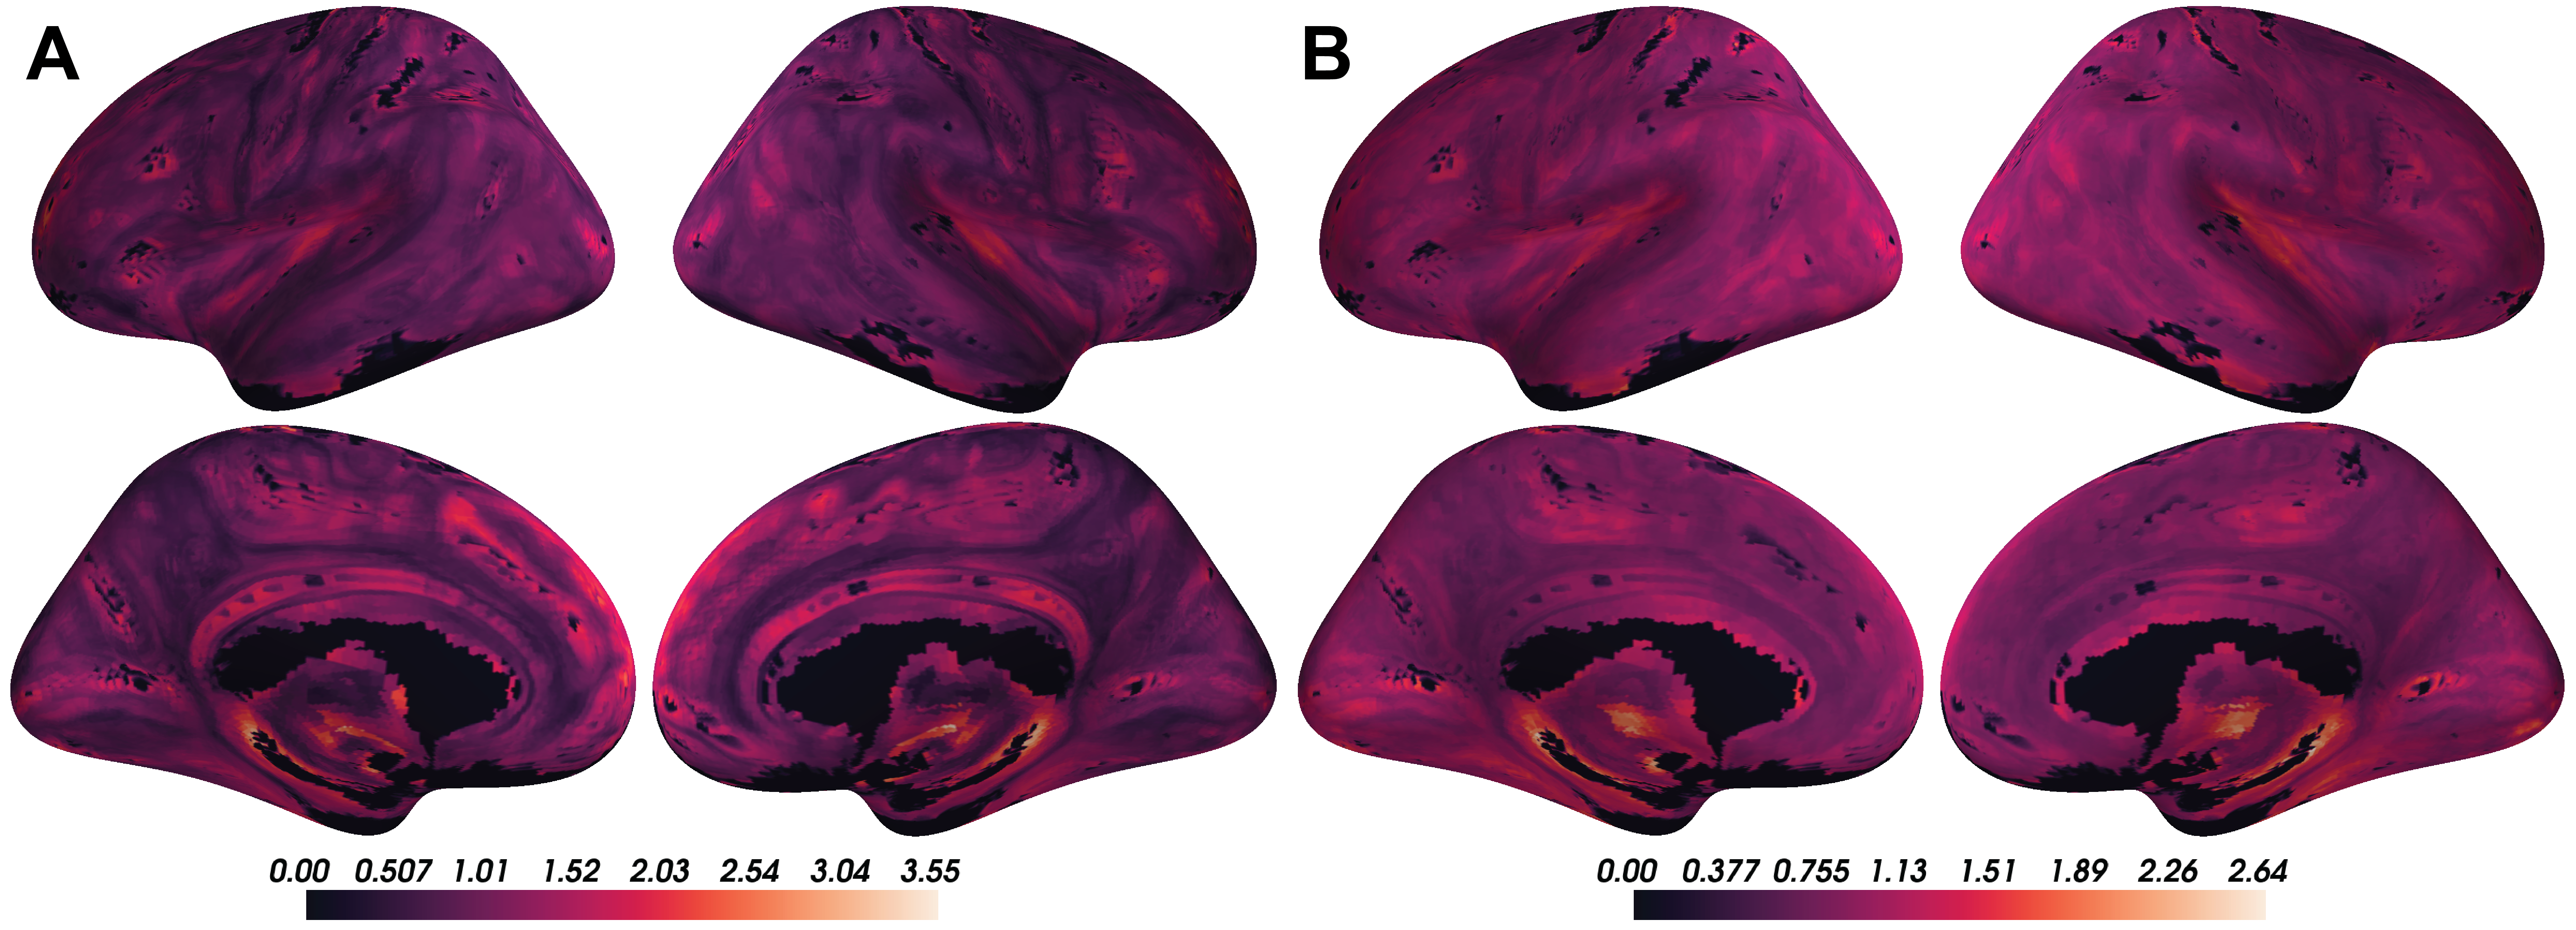
\includegraphics[width=100.01in]{figures/coupling_desc-01} \caption{Test}(\#fig:desc_fig)
\end{figure}

Comparing to the Yeo 7 functional networks, areas of strong coupling are observed primarily in the default and frontoparietal networks. Small portions of the visual network as well as other networks also show strong coupling, though those patterns were less apparent.

These voxel-wise descriptive maps of coupling showed unique information to descriptive maps of each of the individual modalities (TOCITE SUPPLEMENT).

\hypertarget{cbf-alff-reho-coupling-evolves-with-age-throughout-gray-matter-structures}{%
\subsection{CBF-ALFF-ReHo coupling evolves with age throughout gray matter structures}\label{cbf-alff-reho-coupling-evolves-with-age-throughout-gray-matter-structures}}

Linear associations between strength of coupling and age were present in subcortical structures and cortical networks (TOCITE FIG; corrected p \textless{} 0.05). In subcortical structures, age-related changes in CBF-ALFF-ReHo coupling occurred primarily in the caudate and pallidum, though such changes were also observed in sizable proportions of the hippocampus, putamen, and thalamus.

In cortical networks, coupling and age associations were rare in all networks except the frontoparietal and default networks (TOCITE FIG BINARY). These two networks were also the networks in which the average strength of coupling across subjects was highest (TOCITE FIG). Spin testing between functional networks and age-related changes in coupling showed enrichment of coupling and age associations in the frontoparietal (p = 0.013) and default networks (p = 0.039).

\hypertarget{cbf-alff-reho-coupling-varies-between-males-and-females-primarily-in-subcortical-regions}{%
\subsection{CBF-ALFF-ReHo coupling varies between males and females, primarily in subcortical regions}\label{cbf-alff-reho-coupling-varies-between-males-and-females-primarily-in-subcortical-regions}}

Associations between CBF-ALFF-ReHo coupling and sex were present primarily in the hippocampus and thalamus (TOCITE FIG; corrected p \textless{} 0.05). Coupling was rare in other subcortical structures and all functional networks - only 1\% to 3\% of voxels in these regions showed coupling and sex associations (TOCITE FIG BINARY).

Spin testing between functional networks and sex-related changes in coupling revealed enrichment of coupling and sex associations in the frontoparietal network (p = 0.012), despite the small proportion of the frontoparietal network that exhibited coupling associations with sex.

\hypertarget{discussion}{%
\section{Discussion}\label{discussion}}

As growing emphasis is placed on the acquisition multi-modal data, new methodologies are necessary to enable these analyses. In 2016, Vandekar et al.~introduced a method based on local regression slopes to study IMCo relationships at the single voxel level and showed it could reveal patterns between cortical thickness and sulcal depth that had been undiscovered by studies conducted on regions of interest or across the entire cortex \citep{vandekarSubjectlevelMeasurementLocal2016}. Since then, this method for studying local coupling has continued to enable discoveries \citep{ballerDevelopmentalCouplingCerebral2021}. However, despite its strengths, because this method relies on estimating regression slopes between modalities, it is inherently limited to the two-modality setting, cannot take correlation between modalities into account, and is asymmetric.

In this manuscript, we introduce a generalized approach to estimating IMCo that can be applied to two or more modalities, can be interpreted as a direct summary of local covariance matrices, and is symmetric. This method can be used with any combination of volumetric images to produce single-subject, voxel-resolution coupling images which can then be analyzed using standard techniques. We applied this method to show significant coupling between cerebral blood flow, resting state activations, and local connectivity throughout the brain. We then used voxel-level analyses to characterize how coupling varies in neurodevelopment.

\hypertarget{coupling-of-blood-flow-resting-state-activation-and-connectivity-vary-with-age-and-sex}{%
\subsection{Coupling of blood flow, resting state activation, and connectivity vary with age and sex}\label{coupling-of-blood-flow-resting-state-activation-and-connectivity-vary-with-age-and-sex}}

We found CBF-ALFF-ReHo coupling was spatially heterogeneous and varied with age and sex in neurodevelopment in subcortical structures and cortical networks. These findings are unique to those from individual modality analyses, uncovering otherwise undetectable intermodal interactions. We noticed regions with high CBF-ALFF-ReHo coupling across subjects also tended to have high variance in coupling. This suggests these regions may be biologically interesting in the context of CBF-ALFF-ReHo coupling. However, it is uncertain whether this signal is driven by local changes across all subjects, specific subject-level phenotypes, or something else entirely. In future studies, we will investigate such regions further to explain this heterogeneity.

Spin testing showed the high proportion of coupling-age associations in the frontoparietal and default networks were enriched when compared to the cortex overall. This suggests that, not only do vascular organization, resting state activation, and connectivity change individually in neurodevelopment, but the strength of interaction between these features also changes. These findings are consistent with and add to the literature that frontoparietal and default networks are important regions for change in neurodevelopment {[}TOCITE{]}. In subcortical structures, high proportions of coupling associations with age seen in the caudate, pallidum, hippocampus, and thalamus suggest modulation of vascular, resting state activation, and connectivity coupling may be necessary in the development of movement, memory, and fundamental brain activities.

High proportions of coupling associations with sex in the hippocampus and thalamus suggest differences in memory and fundamental brain activities between males and females could be explained in part by the strength of vascular organization, resting state activation, and connectivity coupling. The rarity of coupling-sex associations throughout the cortex suggest this coupling may not play a role in explaining sex-based differences in higher-order processing.

Interestingly, despite low coupling-sex signal in the frontoparietal network, spin testing showed enrichment of coupling associations with sex in this network - since spin testing is a spatial permutation test which uses the sex-coupling association thresholded p-value map to generate data under the null, this is likely due to a combination of overall rare such associations in the cortex and the particular spatial distribution of these associations within the frontoparietal network. This finding highlights potential shortcomings of using the spin test for enrichment analysis. Additionally, statistical analysis of enrichment in subcortical structures is not yet possible. More methods development is needed in this area.

\hypertarget{limitations}{%
\subsection{Limitations}\label{limitations}}

PCA-based IMCo is designed to summarize a complex local covariance structure as one value to allow for easy analysis and data reduction. While this property is a main strength of the method, it leads to outputs that can be challenging to interpret, and these outputs cannot fully characterize the intricacies of coupling. This is especially true in settings with more than two modalities, as the covariance structure becomes even more complex and biological interpretation of coupling between many modalities can be non-intuitive.

The symmetric nature of PCA-based IMCo is conducive to more consistent interpretation when compared to slope-based IMCo. However, while slope is an intuitive measure that can be interpreted as capturing the effect size of a relationship, the generalizable nature of our PCA-based coupling value makes it challenging to interpret biologically. Instead, it is most accurately interpreted in statistical terms - as a measure of the proportion of variance explained by the first eigenvector, or as a measure of how well the local covariance structure can be summarized by the first eigenvector. Here, we chose to interpret neighborhoods whose covariance structures could be well-summarized as ones that are strongly coupled.

This interpretation of PCA-based coupling highlights that in two-modality settings it cannot describe biological directionality of coupling - whether local increases in one modality lead, on average, to increases or decreases in the other modality. In more than two modalities, pairwise directionality is not described. Instead, it can only describe the strength of the coupling relationship. However, this can also be seen as an improvement over slope-based IMCo - with PCA-based IMCo, larger values uniformly correspond to stronger coupling, while with slope-based IMCo, more positive or more negative values both correspond to stronger coupling.

Finally, though PCA-based coupling does not require specification of an arbitrary reference modality to calculate coupling values, it is still subject to other run-time choices, such as FWHM value or application of masks.

\hypertarget{future-directions}{%
\subsection{Future directions}\label{future-directions}}

In this study, we applied PCA-based IMCo to study coupling between features derived from pcASL and rfMRI modalities, but it can be applied in any study where interactions between multiple modalities are of interest. For example, Shokri-Kojori et al.~showed correspondence between cerebral glucose metabolism and fluctuations in blood oxygenation differed between brain networks in healthy patients and was also sensitive to differences related to acute or chronic alcohol use \citep{shokri-kojoriCorrespondenceCerebralGlucose2019}. However, these correspondence analyses were performed regionally or globally - voxel-wise IMCo analyses could reveal further insights.

In the context of neurodegenerative disorders, it is well-known that Alzheimer's disease is characterized by changes in structural and functional MRI as well as in amyloid-tau positron emission tomography (PET) \citep{frisoniClinicalUseStructural2010, rowleyAmyloidTauPET2020, sperlingPotentialFunctionalMRI2011}. Numerous studies have been done to characterize Alzheimer's-related changes in these individual modalities as well as on interactions between these modalities \citep{bucknerMolecularStructuralFunctional2005, hasaniSystematicReviewAssociation2021, renApplicationStructuralFunctional2020, walesEffectsAmyloidTau2021}. In this setting, PCA-based IMCo could provide voxel-level resolution in pairwise comparisons as well as in all three modalities together. This could be useful as a data reduction tool to simplify complex covariance structures for descriptive analyses as well as a data augmentation tool for predictive efforts.

\hypertarget{conclusion}{%
\section{Conclusion}\label{conclusion}}

PCA-based IMCo offers a generalized approach for describing coupling between two modalities and a novel perspective for summarizing the overall covariance structure between more than two modalities. Here, we applied this method to the analysis of coupling between cerebral blood flow, resting state activations, and local connectivity maps. This analysis revealed patterns in neurodevelopment with respect to age and sex that were unique to those present in any individual modality. As multi-modal data becomes more common, we hope that PCA-based IMCo will serve as a tool for capturing complex intermodal relationships and allow for additional descriptive analyses, improved prediction efforts, and novel methodological advances, among others.

\hypertarget{acknowledgements}{%
\section{Acknowledgements}\label{acknowledgements}}

This study was supported by grants from the National Institute of Mental Health (R01MH112847 to TDS and RTS; R01MH120482 and R01MH113550 to TDS; R01 MH123550-01 to RTS; R01MH107235 to RCG; 2T32MH019112-29A1 to EBB; R01MH120174, R01MH119185, and R56AG066656 to DRR). The PNC data used was funded by NIMH RC2 grants (MH089983 and MH089924 to REG).

\hypertarget{references}{%
\section{References}\label{references}}

\hypertarget{refs}{}
\begin{CSLReferences}{0}{0}
\end{CSLReferences}

\hypertarget{appendix-supplementary-materials}{%
\appendix}


  \bibliography{ref.bib,references.bib,packages.bib}

\end{document}
